%%**************************************************************
%% Vorlage fuer Bachelorarbeiten (o.ä.) der DHBW
%%
%% Autor: Tobias Dreher, Yves Fischer
%% Datum: 06.07.2011
%%
%% Autor: Michael Gruben
%% Datum: 15.05.2013
%%
%% Autor: Markus Barthel
%% Datum: 22.08.2014
%%**************************************************************

%!TEX root = ../dokumentation.tex

%
% Nahezu alle Einstellungen koennen hier getaetigt werden
%

\RequirePackage[l2tabu, orthodox]{nag}	% weist in Commandozeile bzw. log auf veraltete LaTeX Syntax hin

\documentclass[%
	pdftex,
	oneside,			% Einseitiger Druck.
	12pt,				% Schriftgroesse
	parskip=half,		% Halbe Zeile Abstand zwischen Absätzen.
%	topmargin = 10pt,	% Abstand Seitenrand (Std:1in) zu Kopfzeile [laut log: unused]
	headheight = 12pt,	% Höhe der Kopfzeile
%	headsep = 30pt,	% Abstand zwischen Kopfzeile und Text Body  [laut log: unused]
	headsepline,		% Linie nach Kopfzeile.
	footsepline,		% Linie vor Fusszeile.
	footheight = 16pt,	% Höhe der Fusszeile
	abstracton,		% Abstract Überschriften
	DIV=calc,		% Satzspiegel berechnen
	BCOR=8mm,		% Bindekorrektur links: 8mm
	headinclude=false,	% Kopfzeile nicht in den Satzspiegel einbeziehen
	footinclude=false,	% Fußzeile nicht in den Satzspiegel einbeziehen
	listof=totoc,		% Abbildungs-/ Tabellenverzeichnis im Inhaltsverzeichnis darstellen
	toc=bibliography,	% Literaturverzeichnis im Inhaltsverzeichnis darstellen
]{scrreprt}	% Koma-Script report-Klasse, fuer laengere Bachelorarbeiten alternativ auch: scrbook

% Einstellungen laden
\usepackage{xstring}
\usepackage[utf8]{inputenc}
\usepackage[T1]{fontenc}

\newcommand{\einstellung}[1]{%
  \expandafter\newcommand\csname #1\endcsname{}
  \expandafter\newcommand\csname setze#1\endcsname[1]{\expandafter\renewcommand\csname#1\endcsname{##1}}
}
\newcommand{\langstr}[1]{\einstellung{lang#1}}

\einstellung{matrikelnr}
\einstellung{titel}
\einstellung{kurs}
\einstellung{datumAbgabe}
\einstellung{firma}
\einstellung{firmenort}
\einstellung{abgabeort}
\einstellung{abschluss}
\einstellung{studiengang}
\einstellung{dhbw}
\einstellung{betreuer}
\einstellung{gutachter}
\einstellung{zeitraum}
\einstellung{arbeit}
\einstellung{autor}
\einstellung{sprache}
\einstellung{schriftart}
\einstellung{seitenrand}
\einstellung{kapitelabstand}
\einstellung{spaltenabstand}
\einstellung{zeilenabstand}
\einstellung{zitierstil}
 % verfügbare Einstellungen
%%%%%%%%%%%%%%%%%%%%%%%%%%%%%%%%%%%%%%%%%%%%%%%%%%%%%%%%%%%%%%%%%%%%%%%%%%%%%%%
%                                   Einstellungen
%
% Hier können alle relevanten Einstellungen für diese Arbeit gesetzt werden.
% Dazu gehören Angaben u.a. über den Autor sowie Formatierungen.
%
%
%%%%%%%%%%%%%%%%%%%%%%%%%%%%%%%%%%%%%%%%%%%%%%%%%%%%%%%%%%%%%%%%%%%%%%%%%%%%%%%


%%%%%%%%%%%%%%%%%%%%%%%%%%%%%%%%%%%% Sprache %%%%%%%%%%%%%%%%%%%%%%%%%%%%%%%%%%%
%% Aktuell sind Deutsch und Englisch unterstützt.
%% Es werden nicht nur alle vom Dokument erzeugten Texte in
%% der entsprechenden Sprache angezeigt, sondern auch weitere
%% Aspekte angepasst, wie z.B. die Anführungszeichen und
%% Datumsformate.
\setzesprache{en} % oder en
%%%%%%%%%%%%%%%%%%%%%%%%%%%%%%%%%%%%%%%%%%%%%%%%%%%%%%%%%%%%%%%%%%%%%%%%%%%%%%%%

%%%%%%%%%%%%%%%%%%%%%%%%%%%%%%%%%%% Angaben  %%%%%%%%%%%%%%%%%%%%%%%%%%%%%%%%%%%
%% Die meisten der folgenden Daten werden auf dem
%% Deckblatt angezeigt, einige auch im weiteren Verlauf
%% des Dokuments.
\setzematrikelnr{5707482}
\setzekurs{TINF14A}
\setzetitel{Influence of Bring Your Own Device and Internet of Things on the security of networks}
\setzedatumAbgabe{September 2017}
\setzefirma{Hewlett Packard GmbH}
\setzefirmenort{Boeblingen}
\setzeabgabeort{Stuttgart}
\setzeabschluss{Bachelor of Science}
\setzestudiengang{Applied Computer Science}
\setzedhbw{Stuttgart}
\setzebetreuer{Andreas Hausmann}
\setzegutachter{Prof. Dr.\ Bernd Schwinn}
\setzezeitraum{12 Wochen}
\setzearbeit{Bachelor thesis}
\setzeautor{David Volz}
%%%%%%%%%%%%%%%%%%%%%%%%%%%%%%%%%%%%%%%%%%%%%%%%%%%%%%%%%%%%%%%%%%%%%%%%%%%%%%%%

%%%%%%%%%%%%%%%%%%%%%%%%%%%% Literaturverzeichnis %%%%%%%%%%%%%%%%%%%%%%%%%%%%%%
%% Bei Fehlern während der Verarbeitung bitte in ads/header.tex bei der
%% Einbindung des Pakets biblatex (ungefähr ab Zeile 110,
%% einmal für jede Sprache), biber in bibtex ändern.
\newcommand{\ladeliteratur}{%
	\addbibresource{bibliographie.bib}
	%\addbibresource{weitereDatei.bib}
}
%% Zitierstil
%% siehe: http://ctan.mirrorcatalogs.com/macros/latex/contrib/biblatex/doc/biblatex.pdf (3.3.1 Citation Styles)
%% mögliche Werte z.B numeric-comp, alphabetic, authoryear
\setzezitierstil{numeric-comp}
%%%%%%%%%%%%%%%%%%%%%%%%%%%%%%%%%%%%%%%%%%%%%%%%%%%%%%%%%%%%%%%%%%%%%%%%%%%%%%%%

%%%%%%%%%%%%%%%%%%%%%%%%%%%%%%%%% Layout %%%%%%%%%%%%%%%%%%%%%%%%%%%%%%%%%%%%%%%
%% Verschiedene Schriftarten
% laut nag Warnung: palatino obsolete, use mathpazo, helvet (option scaled=.95), courier instead
\setzeschriftart{lmodern} % palatino oder goudysans, lmodern, libertine

%% Paket um Textteile drehen zu können
%\usepackage{rotating}
%% Paket um Seite im Querformat anzuzeigen
%\usepackage{lscape}

%% Seitenränder
\setzeseitenrand{2.5cm}

%% Abstand vor Kapitelüberschriften zum oberen Seitenrand
\setzekapitelabstand{20pt}

%% Spaltenabstand
\setzespaltenabstand{10pt}
%%Zeilenabstand innerhalb einer Tabelle
\setzezeilenabstand{1.5}
%%%%%%%%%%%%%%%%%%%%%%%%%%%%%%%%%%%%%%%%%%%%%%%%%%%%%%%%%%%%%%%%%%%%%%%%%%%%%%%%

%%%%%%%%%%%%%%%%%%%%%%%%%%%%% Verschiedenes  %%%%%%%%%%%%%%%%%%%%%%%%%%%%%%%%%%%
%% Farben (Angabe in HTML-Notation mit großen Buchstaben)
\newcommand{\ladefarben}{%
	\definecolor{LinkColor}{HTML}{00007A}
	\definecolor{ListingBackground}{HTML}{FCF7DE}
}
%% Mathematikpakete benutzen (Pakete aktivieren)
%\usepackage{amsmath}
%\usepackage{amssymb}

%% Programmiersprachen Highlighting (Listings)
\newcommand{\listingsettings}{%
	\lstset{%
		language=Java,			% Standardsprache des Quellcodes
		numbers=left,			% Zeilennummern links
		stepnumber=1,			% Jede Zeile nummerieren.
		numbersep=5pt,			% 5pt Abstand zum Quellcode
		numberstyle=\tiny,		% Zeichengrösse 'tiny' für die Nummern.
		breaklines=true,		% Zeilen umbrechen wenn notwendig.
		breakautoindent=true,	% Nach dem Zeilenumbruch Zeile einrücken.
		postbreak=\space,		% Bei Leerzeichen umbrechen.
		tabsize=2,				% Tabulatorgrösse 2
		basicstyle=\ttfamily\footnotesize, % Nichtproportionale Schrift, klein für den Quellcode
		showspaces=false,		% Leerzeichen nicht anzeigen.
		showstringspaces=false,	% Leerzeichen auch in Strings ('') nicht anzeigen.
		extendedchars=true,		% Alle Zeichen vom Latin1 Zeichensatz anzeigen.
		captionpos=b,			% sets the caption-position to bottom
		backgroundcolor=\color{ListingBackground}, % Hintergrundfarbe des Quellcodes setzen.
		xleftmargin=0pt,		% Rand links
		xrightmargin=0pt,		% Rand rechts
		frame=single,			% Rahmen an
		frameround=ffff,
		rulecolor=\color{darkgray},	% Rahmenfarbe
		fillcolor=\color{ListingBackground},
		keywordstyle=\color[rgb]{0.133,0.133,0.6},
		commentstyle=\color[rgb]{0.133,0.545,0.133},
		stringstyle=\color[rgb]{0.627,0.126,0.941}
	}
}
%%%%%%%%%%%%%%%%%%%%%%%%%%%%%%%%%%%%%%%%%%%%%%%%%%%%%%%%%%%%%%%%%%%%%%%%%%%%%%%%

%%%%%%%%%%%%%%%%%%%%%%%%%%%%%%%% Eigenes %%%%%%%%%%%%%%%%%%%%%%%%%%%%%%%%%%%%%%%
%% Hier können Ergänzungen zur Präambel vorgenommen werden (eigene Pakete, Einstellungen)



 % lese Einstellungen

\newcommand{\iflang}[2]{%
  \IfStrEq{\sprache}{#1}{#2}{}
}

\langstr{abkverz}
\langstr{anhang}
\langstr{glossar}
\langstr{deckblattabschlusshinleitung}
\langstr{artikelstudiengang}
\langstr{studiengang}
\langstr{anderdh}
\langstr{von}
\langstr{dbbearbeitungszeit}
\langstr{dbmatriknr}
\langstr{dbkurs}
\langstr{dbfirma}
\langstr{dbbetreuer}
\langstr{dbgutachter}
\langstr{sperrvermerk}
\langstr{erklaerung}
\langstr{abstract}
\langstr{listingname}
\langstr{listlistingname}
\langstr{listingautorefname}
 % verfügbare Strings
\input{lang/\sprache} % Übersetzung einlesen

% Einstellung der Sprache des Paketes Babel und der Verzeichnisüberschriften
\iflang{de}{\usepackage[english, ngerman]{babel}}
\iflang{en}{\usepackage[ngerman, english]{babel}} 


%%%%%%% Package Includes %%%%%%%

\usepackage[margin=\seitenrand,foot=1cm]{geometry}	% Seitenränder und Abstände
\usepackage[activate]{microtype} %Zeilenumbruch und mehr
\usepackage[onehalfspacing]{setspace}
\usepackage{makeidx}
\usepackage[autostyle=true,german=quotes]{csquotes}
\usepackage{longtable}
\usepackage{enumitem}	% mehr Optionen bei Aufzählungen
\usepackage{graphicx}
\usepackage{pdfpages}   % zum Einbinden von PDFs
\usepackage{xcolor} 	% für HTML-Notation
\usepackage{float}
\usepackage{array}
\usepackage{calc}		% zum Rechnen (Bildtabelle in Deckblatt)
\usepackage[right]{eurosym}
\usepackage{wrapfig}
\usepackage{pgffor} % für automatische Kapiteldateieinbindung
\usepackage[perpage, hang, multiple, stable]{footmisc} % Fussnoten
\usepackage[printonlyused]{acronym} % falls gewünscht kann die Option footnote eingefügt werden, dann wird die Erklärung nicht inline sondern in einer Fußnote dargestellt
\usepackage{listings}

% Notizen. Einsatz mit \todo{Notiz} oder \todo[inline]{Notiz}. 
\usepackage[obeyFinal,backgroundcolor=yellow,linecolor=black]{todonotes}
% Alle Notizen ausblenden mit der Option "final" in \documentclass[...] oder durch das auskommentieren folgender Zeile
% \usepackage[disable]{todonotes}

% Kommentarumgebung. Einsatz mit \comment{}. Alle Kommentare ausblenden mit dem Auskommentieren der folgenden und dem aktivieren der nächsten Zeile.
\newcommand{\comment}[1]{\par {\bfseries \color{blue} #1 \par}} %Kommentar anzeigen
% \newcommand{\comment}[1]{} %Kommentar ausblenden


%%%%%% Configuration %%%%%

%% Anwenden der Einstellungen

\usepackage{\schriftart}
\ladefarben{}

% Titel, Autor und Datum
\title{\titel}
\author{\autor}
\date{\datum}

% PDF Einstellungen
\usepackage[%
	pdftitle={\titel},
	pdfauthor={\autor},
	pdfsubject={\arbeit},
	pdfcreator={pdflatex, LaTeX with KOMA-Script},
	pdfpagemode=UseOutlines, 		% Beim Oeffnen Inhaltsverzeichnis anzeigen
	pdfdisplaydoctitle=true, 		% Dokumenttitel statt Dateiname anzeigen.
	pdflang={\sprache}, 			% Sprache des Dokuments.
]{hyperref}

% (Farb-)einstellungen für die Links im PDF
\hypersetup{%
	colorlinks=true, 		% Aktivieren von farbigen Links im Dokument
	linkcolor=LinkColor, 	% Farbe festlegen
	citecolor=LinkColor,
	filecolor=LinkColor,
	menucolor=LinkColor,
	urlcolor=LinkColor,
	linktocpage=true, 		% Nicht der Text sondern die Seitenzahlen in Verzeichnissen klickbar
	bookmarksnumbered=true 	% Überschriftsnummerierung im PDF Inhalt anzeigen.
}
% Workaround um Fehler in Hyperref, muss hier stehen bleiben
\usepackage{bookmark} %nur ein latex-Durchlauf für die Aktualisierung von Verzeichnissen nötig

% Schriftart in Captions etwas kleiner
\addtokomafont{caption}{\small}

% Literaturverweise (sowohl deutsch als auch englisch)
\iflang{de}{%
\usepackage[
	backend=biber,		% empfohlen. Falls biber Probleme macht: bibtex
	bibwarn=true,
	bibencoding=utf8,	% wenn .bib in utf8, sonst ascii
	sortlocale=de_DE,
	style=\zitierstil,
]{biblatex}
}
\iflang{en}{%
\usepackage[
	backend=bibtex,		% empfohlen. Falls biber Probleme macht: bibtex
	bibwarn=true,
	bibencoding=utf8,	% wenn .bib in utf8, sonst ascii
	sortlocale=en_US,
	style=\zitierstil,
]{biblatex}
}

\ladeliteratur{}

% Glossar
\usepackage[nonumberlist,toc]{glossaries}

%%%%%% Additional settings %%%%%%

% Hurenkinder und Schusterjungen verhindern
% http://projekte.dante.de/DanteFAQ/Silbentrennung
\clubpenalty = 10000 % schließt Schusterjungen aus (Seitenumbruch nach der ersten Zeile eines neuen Absatzes)
\widowpenalty = 10000 % schließt Hurenkinder aus (die letzte Zeile eines Absatzes steht auf einer neuen Seite)
\displaywidowpenalty=10000

% Bildpfad
\graphicspath{{images/}}

% Einige häufig verwendete Sprachen
\lstloadlanguages{PHP,Python,Java,C,C++,bash}
\listingsettings{}
% Umbennung des Listings
\renewcommand\lstlistingname{\langlistingname}
\renewcommand\lstlistlistingname{\langlistlistingname}
\def\lstlistingautorefname{\langlistingautorefname}

% Abstände in Tabellen
\setlength{\tabcolsep}{\spaltenabstand}
\renewcommand{\arraystretch}{\zeilenabstand}


\makeglossaries
%!TEX root = ../dokumentation.tex

%
% vorher in Konsole folgendes aufrufen:
%	makeglossaries makeglossaries dokumentation.acn && makeglossaries dokumentation.glo
%

%
% Glossareintraege --> referenz, name, beschreibung
% Aufruf mit \gls{...}
%
\newglossaryentry{Glossareintrag}{name={Glossareintrag},plural={Glossareinträge},description={Ein Glossar beschreibt verschiedenste Dinge in kurzen Worten}}



%\newcommand{\ladeliteratur}{%
%	\addbibresource{bibliographie.bib}
%	%\addbibresource{weitereDatei.bib}
%}

\begin{document}

	% Deckblatt
	\begin{spacing}{1}
		%!TEX root = ../dokumentation.tex

\begin{titlepage}
	\begin{longtable}{p{8.2cm} p{5.4cm}}
		{\raisebox{\ht\strutbox-\totalheight}{
\includegraphics[height=2.5cm]{images/firma-deckblatt.png}}} &
		{\raisebox{\ht\strutbox-\totalheight}{
\includegraphics[height=2.5cm]{images/dhbw.png}}}
	\end{longtable}
	\enlargethispage{20mm}
	\begin{center}
		\vspace*{12mm}	{\LARGE\textbf \titel }\\
		\vspace*{12mm}	{\large\textbf \arbeit}\\
		\vspace*{12mm}	\langdeckblattabschlusshinleitung\\
		\vspace*{3mm}		{\textbf \abschluss}\\
		\vspace*{12mm}	\langartikelstudiengang{} \langstudiengang{} \studiengang\\
    \vspace*{3mm}		\langanderdh{} \dhbw\\
		\vspace*{12mm}	\langvon\\
		\vspace*{3mm}		{\large\textbf \autor}\\
		\vspace*{12mm}	\datumAbgabe\\
	\end{center}
	\vfill
	\begin{spacing}{1.2}
	\begin{tabbing}
		mmmmmmmmmmmmmmmmmmmmmmmmmm             \= \kill
		\textbf{\langdbbearbeitungszeit}       \>  \zeitraum\\
		\textbf{\langdbmatriknr, \langdbkurs}  \>  \matrikelnr, \kurs\\
		\textbf{\langdbfirma}                  \>  \firma, \firmenort\\
		\textbf{\langdbbetreuer}               \>  \betreuer\\
		\textbf{\langdbgutachter}              \>  \gutachter
	\end{tabbing}
	\end{spacing}
\end{titlepage}

	\end{spacing}
	\newpage

	\pagenumbering{Roman}

	% Sperrvermerk
	%!TEX root = ../dokumentation.tex

\thispagestyle{empty}
% Sperrvermerk direkt hinter Titelseite
\section*{\langsperrvermerk}

\vspace*{2em}

\iflang{de}{%
  Die vorliegende {\arbeit} mit dem Titel {\itshape{} \titel{}\/} enthält unternehmensinterne bzw. vertrauliche Informationen der {\firma}, ist deshalb mit einem Sperrvermerk versehen und wird ausschließlich zu Prüfungszwecken am Studiengang {\studiengang} der Dualen Hochschule Baden-Württemberg {\dhbw} vorgelegt. Sie ist ausschließlich zur Einsicht durch den zugeteilten Gutachter, die Leitung des Studiengangs und ggf. den Prüfungsausschuss des Studiengangs bestimmt.  Es ist untersagt,
  \begin{itemize}
  \item den Inhalt dieser Arbeit (einschließlich Daten, Abbildungen, Tabellen, Zeichnungen usw.) als Ganzes oder auszugsweise weiterzugeben,
  \item Kopien oder Abschriften dieser Arbeit (einschließlich Daten, Abbildungen, Tabellen, Zeichnungen usw.) als Ganzes oder in Auszügen anzufertigen,
  \item diese Arbeit zu veröffentlichen bzw. digital, elektronisch oder virtuell zur Verfügung zu stellen. 
  \end{itemize}
Jede anderweitige Einsichtnahme und Veröffentlichung – auch von Teilen der Arbeit – bedarf der vorherigen Zustimmung durch den Verfasser und {\firma}.
}

%http://www.ib.dhbw-mannheim.de/fileadmin/ms/bwl-ib/Downloads_alt/Leitfaden_31.05.pdf

\iflang{en}{%
  The {\arbeit} on hand 
  \begin{center}{\itshape{} \titel{}\/}\end{center} 
   contains internal resp.\ confidential data of {\firma}. It is intended solely for inspection by the assigned examiner, the head of the {\studiengang} department and, if necessary, the Audit Committee \langanderdh{} {\dhbw}. It is strictly forbidden
    \begin{itemize}
    \item to distribute the content of this paper (including data, figures, tables, charts etc.) as a whole or in extracts,
    \item to make copies or transcripts of this paper or of parts of it,
    \item to display this paper or make it available in digital, electronic or virtual form.
    \end{itemize}
  Exceptional cases may be considered through permission granted in written form by the author and {\firma}.
}

\vspace{3em}

\abgabeort, \datumAbgabe
\vspace{4em}

\rule{6cm}{0.4pt}\\
\autor

	\newpage

	% Erklärung
	%!TEX root = ../dokumentation.tex

\thispagestyle{empty}

\section*{\langerklaerung}
% http://www.se.dhbw-mannheim.de/fileadmin/ms/wi/dl_swm/dhbw-ma-wi-organisation-bewertung-bachelorarbeit-v2-00.pdf
\vspace*{2em}

\iflang{en}{%
Ich versichere hiermit, dass ich meine {\arbeit} mit dem Thema: {\itshape \titel } selbstständig verfasst und keine anderen als die angegebenen Quellen und Hilfsmittel benutzt habe. Ich versichere zudem, dass die eingereichte elektronische Fassung mit der gedruckten Fassung übereinstimmt. 

% https://www.dhbw-karlsruhe.de/fileadmin/user_upload/dokumente/T-Informatik/Prüfungsordnung-Technik-2015-09-29.pdf (S. 19)


% Ich erkläre hiermit ehrenwörtlich: \\
% \begin{enumerate}
% \item dass ich meine {\arbeit} mit dem Thema
% {\itshape \titel } ohne fremde Hilfe angefertigt habe;
% \item dass ich die Übernahme wörtlicher Zitate aus der Literatur sowie die Verwendung der Gedanken
% anderer Autoren an den entsprechenden Stellen innerhalb der Arbeit gekennzeichnet habe;
% \item dass ich meine {\arbeit} bei keiner anderen Prüfung vorgelegt habe;
% \item dass die eingereichte elektronische Fassung exakt mit der eingereichten schriftlichen Fassung
% übereinstimmt.
% \end{enumerate}
% 
% Ich bin mir bewusst, dass eine falsche Erklärung rechtliche Folgen haben wird.

% % http://www.ib.dhbw-mannheim.de/fileadmin/ms/bwl-ib/Downloads_alt/Leitfaden_31.05.pdf (S. 52)
}


\iflang{de}{%
Hereby I solemnly declare:
\begin{enumerate}
\item that this {\arbeit}, titled {\itshape \titel } is entirely the product of my own scholarly work, unless otherwise indicated in the text or references, or acknowledged below;
\item I have indicated the thoughts adopted directly or indirectly from other sources at the appropriate places within the document;
\item this {\arbeit} has not been submitted either in whole or part, for a degree at this or any other university or institution;
\item I have not published this {\arbeit} in the past; 
\item the printed version is equivalent to the submitted electronic one.
\end{enumerate}
I am aware that a dishonest declaration will entail legal consequences.
}

\vspace{3em}

\abgabeort, \datumAbgabe
\vspace{4em}

\rule{6cm}{0.4pt}\\
\autor

	\newpage

	% Abstract
	%!TEX root = ../dokumentation.tex

\pagestyle{empty}

\iflang{de}{%
% Dieser deutsche Teil wird nur angezeigt, wenn die Sprache auf Deutsch eingestellt ist.
\renewcommand{\abstractname}{\langabstract} % Text für Überschrift

% \begin{otherlanguage}{english} % auskommentieren, wenn Abstract auf Deutsch sein soll
\begin{abstract}
Abstract normalerweise auf Englisch. Siehe:  \url{http://www.dhbw.de/fileadmin/user/public/Dokumente/Portal/Richtlinien_Praxismodule_Studien_und_Bachelorarbeiten_JG2011ff.pdf} (8.3.1 Inhaltsverzeichnis)

Ein "`Abstract"' ist eine prägnante Inhaltsangabe, ein Abriss ohne Interpretation und Wertung einer wissenschaftlichen Arbeit. In DIN 1426 wird das (oder auch der) Abstract als Kurzreferat zur Inhaltsangabe beschrieben.

\begin{description}
\item[Objektivität] soll sich jeder persönlichen Wertung enthalten
\item[Kürze] soll so kurz wie möglich sein
\item[Genauigkeit] soll genau die Inhalte und die Meinung der Originalarbeit wiedergeben
\end{description}

Üblicherweise müssen wissenschaftliche Artikel einen Abstract enthalten, typischerweise von 100-150 Wörtern, ohne Bilder und Literaturzitate und in einem Absatz.

Quelle: \url{http://de.wikipedia.org/wiki/Abstract} Abgerufen 07.07.2011

Diese etwa einseitige Zusammenfassung soll es dem Leser ermöglichen, Inhalt der Arbeit und Vorgehensweise
des Autors rasch zu überblicken. Gegenstand des Abstract sind insbesondere 
\begin{itemize}
\item Problemstellung der Arbeit,
\item im Rahmen der Arbeit geprüfte Hypothesen bzw. beantwortete Fragen,
\item der Analyse zugrunde liegende Methode,
\item wesentliche, im Rahmen der Arbeit gewonnene Erkenntnisse,
\item Einschränkungen des Gültigkeitsbereichs (der Erkenntnisse) sowie nicht beantwortete Fragen. 
\end{itemize}
Quelle: \url{http://www.ib.dhbw-mannheim.de/fileadmin/ms/bwl-ib/Downloads_alt/Leitfaden_31.05.pdf}, S.~49
\end{abstract}
% \end{otherlanguage} % auskommentieren, wenn Abstract auf Deutsch sein soll
}



\iflang{en}{%
% Dieser englische Teil wird nur angezeigt, wenn die Sprache auf Englisch eingestellt ist.
\renewcommand{\abstractname}{\langabstract} % Text für Überschrift

\begin{abstract}
An abstract is a brief summary of a research article, thesis, review, conference proceeding or any in-depth analysis of a particular subject or discipline, and is often used to help the reader quickly ascertain the paper's purpose. When used, an abstract always appears at the beginning of a manuscript, acting as the point-of-entry for any given scientific paper or patent application. Abstracting and indexing services for various academic disciplines are aimed at compiling a body of literature for that particular subject.

The terms précis or synopsis are used in some publications to refer to the same thing that other publications might call an ``abstract''. In ``management'' reports, an executive summary usually contains more information (and often more sensitive information) than the abstract does.

Quelle: \url{http://en.wikipedia.org/wiki/Abstract_(summary)}

\end{abstract}
}
	\newpage

	\pagestyle{plain}		% nur Seitenzahlen im Fuß
	
	\RedeclareSectionCommand[beforeskip=\kapitelabstand         ]{chapter} % stellt Abstand vor Kapitelüberschriften ein

	% Inhaltsverzeichnis
	\begin{spacing}{1.1}
		\begingroup
		
			% auskommentieren für Seitenzahlen unter Inhaltsverzeichnis
			\renewcommand*{\chapterpagestyle}{empty}
			\pagestyle{empty}
			
			
			\setcounter{tocdepth}{1}
			%für die Anzeige von Unterkapiteln im Inhaltsverzeichnis
			%\setcounter{tocdepth}{2}
			
			\tableofcontents
			\clearpage
		\endgroup
	\end{spacing}
	\newpage

	% Abkürzungsverzeichnis
	\cleardoublepage
	%!TEX root = ../dokumentation.tex

\addchap{\langabkverz}
%nur verwendete Akronyme werden letztlich im Abkürzungsverzeichnis des Dokuments angezeigt
%Verwendung: 
%		\ac{Abk.}   --> fügt die Abkürzung ein, beim ersten Aufruf wird zusätzlich automatisch die ausgeschriebene Version davor eingefügt bzw. in einer Fußnote (hierfür muss in header.tex \usepackage[printonlyused,footnote]{acronym} stehen) dargestellt
%		\acs{Abk.}   -->  fügt die Abkürzung ein
%		\acf{Abk.}   --> fügt die Abkürzung UND die Erklärung ein
%		\acl{Abk.}   --> fügt nur die Erklärung ein
%		\acp{Abk.}  --> gibt Plural aus (angefügtes 's'); das zusätzliche 'p' funktioniert auch bei obigen Befehlen
%	siehe auch: http://golatex.de/wiki/%5Cacronym
%	
\begin{acronym}[YTMMM]
\setlength{\itemsep}{-\parsep}

\acro{AGPL}{Affero GNU General Public License}
\acro{WSN}{Wireless Sensor Network}
\acro{MANET}{Mobile wireless Ad-hoc NETwork}
\acro{MAC}{Multiple Access Control}
\acro{QoS}{Quality of Service}
\acro{DSR}{Dynamic Source Routing}
\acro{API}{Application Programming Interface}
\acro{WYSIWYG}{What You See Is What You Get}
\acro{HTML}{HyperText Markup Language}
\end{acronym}


	% Abbildungsverzeichnis
	\cleardoublepage
	\listoffigures

	%Tabellenverzeichnis
	\cleardoublepage
	\listoftables

	% Quellcodeverzeichnis
	\cleardoublepage
	\lstlistoflistings
	\cleardoublepage

	\pagenumbering{arabic}
	
	\pagestyle{headings}		% Kolumnentitel im Kopf, Seitenzahlen im Fuß

	% Inhalt
%	\foreach \i in {01,02,03,04,05,06,07,08,09,...,99} {%
%		\edef\FileName{content/\i kapitel}%
%			\IfFileExists{\FileName}{%
%				\input{\FileName}
%			}
%			{%
%				%file does not exist
%			}
%	}

	\chapter{Introduction}
Bring Your Own Device (BYOD) and the Internet of Things (IoT) are both emerging concepts in today's business. While employees bring more and more devices with BYOD to the companies network, IoT introduces equipment, which was not necessarily build for networks. Both concepts introduce security issues to the network 
	\chapter{Internet of Things (IoT)}

The \textit{Internet of Things} is the idea of connecting every device that creates data in any way. Even things that initially were not made for connectivity. For example heaters, windows, doors, lights and fridges. The data gets analysed and evaluated, such that a controller can adjust other devices as needed. \\
The idea of a smart home, which automatically regulates the temperature, light and orders new groceries when needed, can be realized by connecting everything within a house. The light is automatically turned off if nobody is at home, the heater is turned on if it gets too cold and groceries are ordered if the fridge detects a low amount of food.  \\
Advantages the \textit{Internet of Things} has for consumer and producer are listed here:
\begin{itemize}
	 \item The connectivity to other devices can enhance the features and usability of the device. For example, in a smart home a single photo sensor, which measures how much light is within a room, does not do much. But if it is connected to a controller, a motion sensor and the lights, it is possible to automatically turn on the lights, whenever somebody is in the dark room. 
	 \item Another usage of \textit{IoT} is to customize devices. If we stay with the example of our smart home and look at the photo sensor the user might want to change the sensitivity of the sensor. With IoT it is possible to access the sensor (or controller depending on the setup) via the internet and change the sensitivity, instead of physically accessing it.
	 \item By connecting the internet and not just to the local network, two other possibilities arise:
	 \begin{enumerate}
	 	\item The user can access the devices from anywhere. Whenever he has access to the internet he can access his devices. This makes it, for example, possible to turn off the lights, when the user is not at home and has no physical access to his home network. 
	 	\item But not only the user can access the device, but also the producer. This is useful, if the producer analyses the usage data to enhance the product. This makes it possible to fix bugs, make corrections to hardware, schedule maintenance downtime, based on when the device is least used and improve features, which are most often used by the users. This overall increases the lifespan of the product and the satisfaction of the customer. \\
	 	However, this can also come with security risks, which are briefly described in the next chapter among others.  
	 \end{enumerate}
\end{itemize}


\section{Issues}
Even if \textit{IoT} can come with some advantages it also can have some disadvantages. By bringing more and more devices into a network it is hard for the network administrator to keep track of every device. This makes it possible for attackers to bring their own device into the network. But in most cases they do not need to get physical access to the network, since many devices do not have the security standards like most laptops or smartphones have. Together with the sheer amount of different devices \textit{IoT} brings to the network attackers are likely to find some sort of exploit, which grants them access to the network. \\
But not only attackers can be dangerous for companies, but also the producer of some devices. By analysing the usage data they may get confidential data, which their product uses. If for example a network switch breaks down it may be possible that the network traffic is sent to producer. Within this traffic there might be confidential data, which can be harmful for the company or even illegal. Also there is the possibility that the producer is compromised by hackers, which are then able to get more information of the company, making it more vulnerable to their attacks. \\
Lately a botnet named mirai demonstrated, how weak the security of IoT devices can be. It was discovered in August 2016 and consists of only IoT devices. Mirai is capable of DDoS attacks with 1TB/s traffic.

	\chapter{Bring your own Device (BYOD)}
In today's business, many employees want to work on their own device. Whether it is to be mobile or just to have more familiarity to the platform used, the employer has to react to this trend. There are many reasons for employees to use their own device. Those include for example an increased level of comfort, the proficiency with only one device and the use of mobile devices in the first place. \\
The increased level in comfort comes from the familiarity with the devices the employee uses due to the fact that they use the same device privately as well as at work. And since many people are always online with any device it is possible to work anywhere and anytime instead of being bound to the office and fix work hours. \\
In many companies not every employee is entitled to receive a mobile device for work. Only those with a certain position, where it is needed to be able to work on the go. With BYOD it is possible for every other employee to work on their own mobile device instead. Which in turn can increase their productivity, customize their working hours and give freedom for their work place.\\


\section{Device Provisioning}
There are different strategies to provide Devices for the employees. Each varies in enterprise control and Employee Satisfaction. The strategies can be divided into 4 concepts. \parencite{KumarGajar.2013}
\begin{enumerate}
	\item Here's your own Device (HYOD) \\
	With this concept the company decides on everything regarding the device. From the buying process over the installation, configuration and support to the disposal of the device, everything is managed by the company, giving full control and oversight over the life cycle of every device. Whereas the employees has no control except for minor customization options and applications.  \parencite{KumarGajar.2013}
	
	\item Choose your own Device (CYOD) \\
	This approach gives the employee some choice for the device he gets from the company. The company gives the employee a selection of different pre-chosen devices. This gives some options when it comes to manufacturer, operating system and hardware specifications. The pre-selection as well as installation and set-up are still responsibilities of the company. The support is more complicated, since the IT help desk needs to be proficient with all offered equipment. Company-wide software also needs to run on every device which leads to higher implementation overhead and costs. \parencite{KumarGajar.2013}
	
	\item Bring your own Device (BYOD) \\
	Bring your own Device is the concept of using existing private devices in a work environment. Alternatively the company can provides financial help for the employee to buy a device. This allows the employee to freely choose the device, like operating system, manufacturer and hardware specification. This also includes the type, i.e. Desktop Computer, Laptop, Workstation, Tablet, Smartphone, of the device. If he wants to, he can also use multiple different devices. Since the device is owned by the employee, he has most control over it. However, the company can introduce policies since the employee works with (often confidential) company data. Support can often only be provided on a basic level, since every employee can have a different device and to provide expertise for all of them is too expensive to be economical. \parencite{KumarGajar.2013}
	
	\item On your own Device (OYOD) \\
	On your own Device takes it a step further and gives Employees all the freedom he can get. Not even Policies are put in place by the company, making it the option with highest employee satisfaction, but with the lowest enterprise control. \parencite{KumarGajar.2013}
\end{enumerate}
These 4 concepts are not a strict representation of all possibilities. For example, it is possible to give the employee a choice of operating system, while having only one device. This combines both HYOD and CYOD. That's why every company should consider BYOD besides their current strategy, enabling employees to use their own devices alongside any other device. Chances are they are already using it despite it being not officially supported or even allowed. \parencite{IBMSecurity.2016}. But with no BYOD policies in place it is more like OYOD. As seen in the figure \ref{fig:control_v_satisfaction} below, OYOD does not allow any control over the device, which makes it a potential security issue.
\begin{figure}[H]
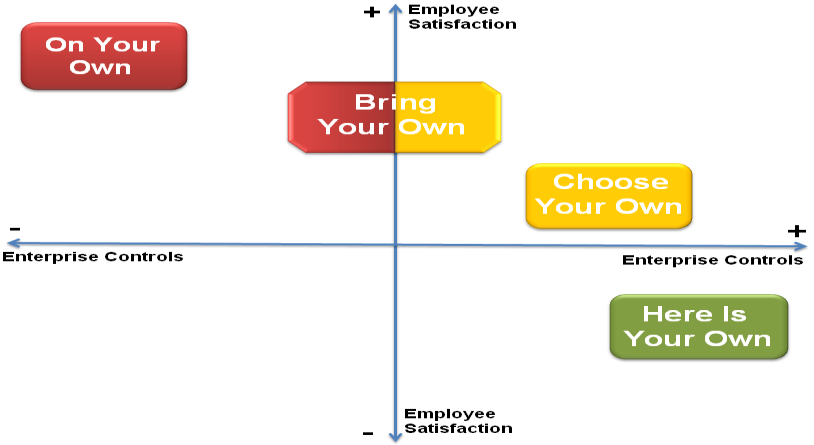
\includegraphics[width=0.7\linewidth]{images/control_v_satisfaction}
\caption{Enterprise Control and Employee Satisfaction of provision strategies \parencite{KumarGajar.2013}}
\label{fig:control_v_satisfaction}
\end{figure}

\section{Architectural Concepts}
There are different technological approaches for using BYOD in a company. Figure \ref{fig:architectural_concepts} shows how company applications can be used from an end user device. The different approaches are compared between presentation, application execution, application launch and data storage. While most of the approaches do not need to store the data on the device, it can be done to optimize network or hardware usage \parencite{Disterer.2013}
\begin{figure}[H]
	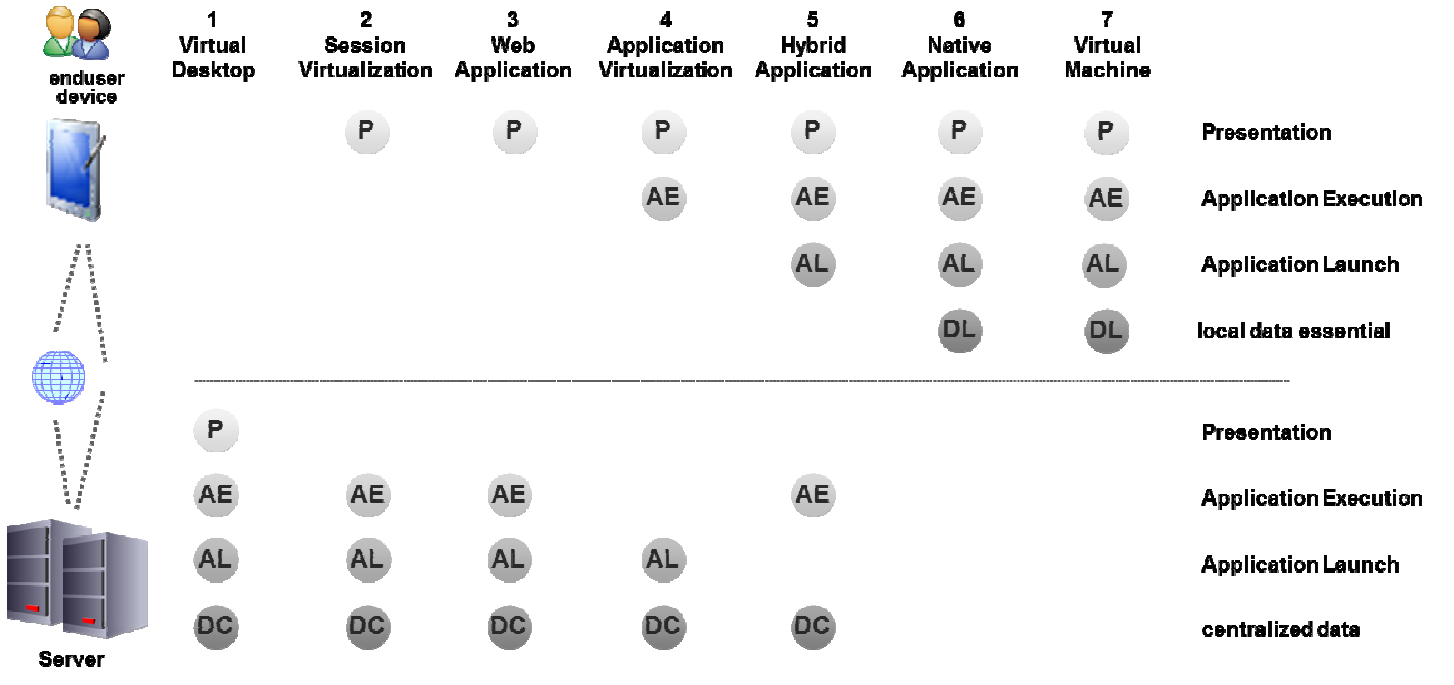
\includegraphics[width=1\linewidth]{images/architectural_concepts}
	\caption{Architectural Concepts and Technological Approaches \parencite{Disterer.2013}}
	\label{fig:architectural_concepts}
\end{figure}
\begin{enumerate}
	\item Virtual Desktop \\
	The employee device launches a virtual machine on a server in the company's network. Every part of the application runs on the server, even the presentation. This makes it the mobile equivalent to a terminal server. As with terminals, all the information for the presentation and user input is sent over the network. However, with a stationary terminal bandwidth is not such a big problem as with mobile devices, which makes this approach not feasible for the time being.  \parencite{Disterer.2013}
	\item Session Virtualization \\
	In \textit{session virtualization}, the client also starts an application on a server in the company's network. The execution and data storage is all done by the server, but the user interface is created on the client device. This reduces the bandwidth, since the client does not need as much information to create the user interface as the \textit{virtual desktop} does to provide the interface itself. Since the end user device creates the interface, the look \& feel and the control scheme can be device specific. This however requires additional implementation effort for each device. \parencite{Disterer.2013}
	\item Web Application \\
	With pure HTML \& CSS this is a special kind of \textit{session virtualization}. If the HTML is extended by JavaScript or some enhanced HTML5 functions, this is considered a \textit{Hybrid Application} instead of a \textit{session virtualization}. Nowadays \textit{web applications} are widely used in many areas. There is a great number of implementations of the standard. For virtually every device there is a browser, which can display the information from the web server. Compared to \textit{virtual desktops} and other \textit{session virtualizations} the bandwidth used is low, making it a better solution for mobile devices. \\
	While the use of a standardized solution is a big advantage for the most part, it also can have disadvantages. For example there is more malware for widely spread software. Another disadvantage is that modern browser access the local system and store potentially confidential data on the device, which poses a security risk. \parencite{Disterer.2013}
	\item Application Virtualization \\
	As seen in Figure \ref{fig:appVirtual} below, in \textit{Application Virtualization} the applications run in an emulator instead of just on top of the operating system. The functions of the operating system are emulated for the application. \parencite{Husain.2008} This has the advantage that the application does not have to be developed for multiple systems. If a new system gets released or an old system gets updated, the developers only need to change the emulator but not all the applications that are supposed to run on that system. With this approach applications often run in separate sandboxes/containers. The applications therefore are isolated from other software running on the device. This reduces the risk of another software interfering with the application as well as preventing it from accessing personal data on the device. \parencite{Disterer.2013}
	\begin{figure}[H]
		\includegraphics[width=1\linewidth]{images/appVirtual}
		\caption{Application running in a native environment and an application virtualization environment \parencite{Egmason.2011}}
		\label{fig:appVirtual}
	\end{figure}
	\item Hybrid Application \\
	\textit{Hybrid Applications} combine \textit{Session Virtualization} with \textit{Native Applications}. The most widespread example are web applications. Locally JavaScript and HTML can execute some parts of the application and the other part is executed on the web server. For the most part \textit{hybrid applications} should be considered as \textit{native applications} when it comes to security  \parencite{Disterer.2013}
	\item Native Application \\
	 \parencite{Disterer.2013}
	\item Virtual Machine \\
	 \parencite{Disterer.2013}
\end{enumerate}

\section{Disadvantages}

\section{Risks}

	\chapter{Setup}
To demonstrate a solution for the issues of IoT and BYOD a example network is created. It is used to show how to effectively add unknown devices to a corporate network and how the devices interact in the network. Afterwards this setup will be integrated into the existing network of the Customer Technology Center (CTC) at Hewlett Packard Enterprise in Boeblingen to make it accessible to HPE's customers. 

\section{Infrastructure}
\subsection{Hardware}

\begin{enumerate}
	\item Switch \\
	All the described Hard- and Software is connected by a Switch via Ethernet. In this case it is an \textit{Aruba Switch 2920-24G-POE+} with 24 Ethernet ports. Power over Ethernet (POE) makes it possible to power the network devices, without additional power infrastructure.
	\item Controller \\
	The controller manages the access points, the WiFi, and all the devices within the network. For this demonstration the controller used is the \textit{Aruba Mobility Controller 7005}. 
	\item Access Points \\
	The access points broadcast the WiFi-signal and act as immediate gateway for the connected devices. In this example network three \textit{Aruba Access Points 305} are used.
	\item Server \\
	A mobile workstation is used as the server for the demonstration. Multiple virtual machines are used to run the different applications. Later in the CTC an HPE server will be used. It runs all necessary applications, like an onboarding and AAA-Server.
\end{enumerate}

\subsection{Software}
The server in the network is running mainly two applications. 
\begin{enumerate}
	\item AAA-Server \\
	As Authentication, Authorization, and Accounting Server \textit{Aruba AirWave} is used. 
	\item Onboarding Server \\
	As an onboarding server \textit{Aruba ClearPass} is used to manage all devices from any guest, employee and any IoT device.. 
\end{enumerate}


\section{Devices}
\begin{enumerate}
	\item Convenience Store \\
	A basic setup for a \textit{convenience store} is provided by the \textit{SNAP PAC Learning Center} from \textit{Opto 22}. It has a control board, some control displays and controllers. With the control board, a fuel tank, a freezer door, a photo sensor and an alarm can be simulated. These input signals are processed by the controllers and then the forwarded to the displaying components. These components are a dial to display the current level of the fuel tank, LED lights to show the current state of the \textit{convenience store} and a speaker to give audio feedback. The main controller offers an API to connect to, to make the information accessible from the internet. With this it is possible, to turn any device into an IoT device.
	\item BYOD \\
	To simulate a BYOD device any smartphone or laptop can be used. 
	\item Camera \\
	The \textit{Wansview IP Security Camera K1} is used as a standard IoT device. In contrast to the \textit{convenience store}, the IP camera represents an IoT device, which is common in modern networks.  
	\item Raspberry Pi \\
	Test123
\end{enumerate}
	\chapter{Device Onboarding}

\section{Convenience Store}

\section{BYOD}

\section{Camera}

\section{Raspberry Pi}
	\chapter{Security}
AAA
\section{Native IP}

\section{Analogue}

\section{Threat}



Policy Based
Rule Based
	\chapter{Implementation}


	\chapter{Conclusion}


	\clearpage

	% Literaturverzeichnis
	\cleardoublepage
	\printbibliography

	% Glossar
	\printglossary[style=altlist,title=\langglossar]
	
	% sonstiger Anhang
	\clearpage
	\appendix
	%% !TeX root = ../dokumentation.tex

\addchap{\langanhang}

(Beispielhafter Anhang)
 

{\Large
\begin{enumerate}[label=\Alph*.]
	\item Assignment
	\item List of CD Contents
	\item CD 
\end{enumerate}
}
\pagebreak
%\includepdf[pages=-,scale=.9,pagecommand={}]{Aufgabenstellung.pdf} % PDF um 10% verkleinert einbinden --> Kopf- und Fußzeile  werden so korrekt dargestellt. Die Option `pages' ermöglicht es, eine bestimmte Sequenz von Seiten (z.B. 2-10 oder `-' für alle Seiten) auszuwählen.
\pagebreak
\section*{B. List of CD Contents}
\begin{tabbing}
	mm \= mm \= mmmmmmmmmmmmmmmm \= \kill
	$\vdash$ \textbf{Literature/} \\ 
	| \> $\vdash$ \textbf{Citavi-Project(incl pdfs)/} \> \> $\Rightarrow$ \textit{Citavi (bibliography software) project with}\\
	| \> | \> \> \textit{almost all found sources relating to this report.} \\
	| \> | \> \> \textit{The PDFs linked to bibliography items therein} \\
	| \> | \> \> \textit{are in the sub-directory `CitaviFiles'}\\
	| \> | \>  -- bibliography.bib  \> $\Rightarrow$ \textit{Exported Bibliography file with all sources}\\
	| \> | \>  --	Studienarbeit.ctv4  \>  $\Rightarrow$ \textit{Citavi Project file}\\
	| \> | \>  $\vdash$ \textbf{CitaviCovers/} \>  $\Rightarrow$ \textit{Images of bibliography cover pages}\\
	| \> | \>  $\vdash$ \textbf{CitaviFiles/} \> $\Rightarrow$ \textit{Cited and most other found PDF resources}\\ %\llcorner
	| \> $\vdash$ \textbf{eBooks/} \\
	| \> $\vdash$ \textbf{JournalArticles/} \\
	| \> $\vdash$ \textbf{Standards/}\\
	| \> $\vdash$ \textbf{Websites/} \\ %\llcorner
	|\\
	$\vdash$ \textbf{Presentation/} \\
	| \>  --presentation.pptx\\
	| \>  --presentation.pdf\\
	|\\
	$\vdash$ \textbf{Report/} \\ %\llcorner
	\>  -- Aufgabenstellung.pdf\\
	\>  -- Studienarbeit2.pdf\\
	\>  $\vdash$ \textbf{Latex-Files/}   $\Rightarrow$ \textit{editable \LaTeX~files and other included files for this report}\\ %\llcorner
	\> \>  $\vdash$  \textbf{ads/}   	\> $\Rightarrow$ \textit{Front- and Backmatter}\\
	\> \>  $\vdash$  \textbf{content/}  \> $\Rightarrow$ \textit{Main part}\\
	\> \>  $\vdash$  \textbf{images/}   \> $\Rightarrow$ \textit{All used images}\\
	\> \>  $\vdash$  \textbf{lang/}  \> $\Rightarrow$ \textit{Language files for \LaTeX~template}\\ %\llcorner
\end{tabbing}

	
\end{document}
